\section{Sterowanie ekranem}
\label{sec:component-controll-remote-screen} % marker umożliwiający odwolanie z sekcji architektura

\subsection{Wstęp}

Klient to komputer podłączony bezpośrednio do ekranu wyświetlającego obraz. Istotnymi cechami takiego urządzenia są przede wszystkim:
\begin{itemize}
	\item niska cena
	\item wystarczająca moc obliczeniowa do uruchomienia przeglądarki, oraz prostej gry w technologi Flash, lub HTML5
	\item duża dostępność
	\item mały rozmiar
\end{itemize}

Głównym zadaniem klientów jest komunikacja serwerem poprzez sieć Ethernet w celu wyświetlania obrazu na podłączonym do klienta ekranie, oraz możliwość sterowania urządzeniami wejścia (klawiatura, myszka) poprzez udostępniony interfejs w sieci Ethernet.


\subsection{Hardware}

\subsubsection{Architektura procesora}
Jeśli chodzi o wybór architektury procesora wybór był całkiem prosty, za sprawą sporej liczby dostępnych urządzeń dostępnych w tej architekturze (32 bitowa architektura ARM\footnote{Advanced RISC Machine} jest najczęściej stosowaną architekturą w urządzeniach mobilnych\cite{acm}), jak i uzasadnioną ich popularnością. Architektura ARM cechuje cię niskim poborem energii, dużą niezawodnością w systemach wbudowanych, oraz dla praktycznie wszystkich dostępnych na rynku procesorów możliwością instalacji w pełni funkcjonalnego systemu operacyjnego.
Procesory oparte o architekturę ARM przetwarzają instrukcje z wykorzystaniem mechanizmu potokowania. Procesor może wykonywać trzy rodzaje instrukcji:
\begin{itemize}
	\item 32-bitowe ARM
	\item 64-bitowe ARM (Apple A7)
	\item 16-bitowe Thumb (oraz Thumb2)
\end{itemize}

\\
Firma ARM projektuje rdzenie procesorów i sprzedaje je producentom. Producenci z kolei tworzą urządzenia typu SoC\footnote{System on Chip} - dodawane są bloki funkcyjne, jednostki wektorowe czy procesory sygnałowe. Istnieje też spora lista firm, które projektują swoje rdzenie wykorzystujące zbiór instrukcji ARM m.in. Apple, XScale, czy Faraday.
\\
Istotną cechą, którą powinien posiadać procesor ARM jest jednostka MMU\footnote{Memory Managment Unit}. Jest to jednostka odpowiadająca za dostęp do zewnętrznej pamięci, translacje adresu wirtualnego na fizyczny, oraz kontroli uprawnień dostępu do pamięci. Wiele rdzeni ARM nie jest wyposażonych w tą jednostkę, która staje się obligatoryjna podczas gdy chcemy zainstalować system operacyjny Linux. 
\\

Po wyborze architektury procesora należy wybrać rodzinę procesora. Rodzina Cortex jest kolejną generacją procesorów po ARM7, ARM9, czy ARM11.

\begin{figure}
\begin{center}
	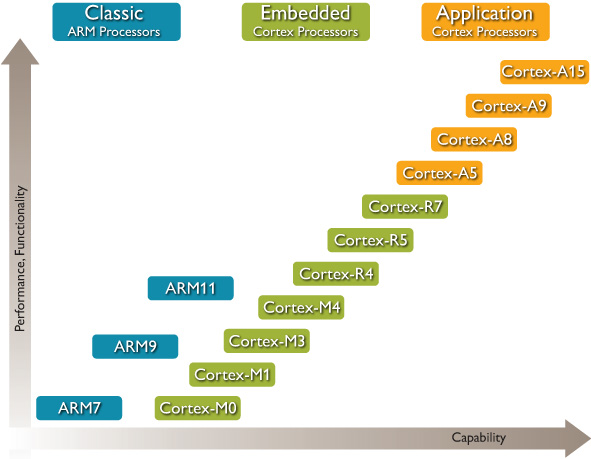
\includegraphics[scale=0.6]{ARM_Comparison}
\end{center}
\caption{Porównanie rodzin architektury ARM}
\label{fig:ARM_Comp}
\end{figure}

Zgodnie z tym co można zauważyć na rysunku~\ref{fig:ARM_Comp} architektura Cortex jest rodziną cechującą się wyższym od swoich poprzedników współczynnikiem wydajności na cykl zegara i niższym zużyciem energii.

Na rynku można wyodrębnić 3 główne chipy bazujące na architekturze ARM:
\begin{itemize}
	\item Allwinner (sunxi)
	Przykładowe produkty:
	\begin{itemize}
		\item Hackberry A10
		\item MK802
	\end{itemize}

	Chipy Allwinnera charakteryzują się stosunkowo najniższą ceną, oba przedstawione wyżej modele bazują na rdzeniu Cortex-A8 taktowane zegarem 1GHz, oraz dysponujące 1GB pamięci operacyjnej. Wyposażone są także w procesor graficzny ARM Mali 400
	
	\item Freescale i.MX6 (imx)
	Przykładowe produkty:
	\begin{itemize}
		\item MarS
		\item IMX53QSB
	\end{itemize}
	\item TI OMAP3/4
	Przykładowe produkty:
		\begin{itemize}
			\item Beaglebone Black
			\item Panda Board
		\end{itemize}
	Ta rodzina zyskała bardzo dużą popularność. Chipy OMAP3 wyposażone są w zmiennoprzecinkową jednostkę oraz zestaw instrukcji wektorowych NEON. Główną cechą tego rozwiązania jest dużo wydajność operacji przy zachowaniu prostoty ich programowania.
\end{itemize}



\subsection{System operacyjny Linux}

Nie dysponując zbyt dużą mocą obliczeniową, małą pamięcią operacyjną, oraz niewielką przestrzenią dyskową należy dobrze dobrać, oraz skonfigurować system operacyjny. Do tego celu wybrano dystrybucje linuksa - Debian. Cechuje się ona przede wszystkim wysoką stabilnością (bardzo często wybierana jako system serwerowy), oraz sporą społecznością programistów rozwijających tą dystrybucje co przekłada się na mnogość dostępnych pakietów przygotowanych specjalnie dla tej wersji systemu Linux. Wreszcie system Debian jest wysoce konfigurowalny - oparty o jądro Linux, daje użytkownikowi możliwość zbudowania systemu od podstaw.

Do zbudowania systemu Linux opartego o architekturę ARM posłużono się istniejącą instalacją Debian na komputerze osobistym. 

\subsubsection{Przygotowanie bazowej wersji systemu}

\begin{figure}
\begin{center}
    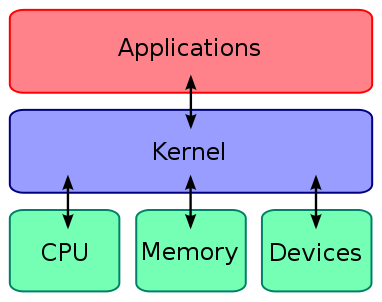
\includegraphics[scale=1]{kernel}
\end{center}
\caption{Działanie jądra systemu Linux}
\label{fig:kernel}
\end{figure}

Jądro \footnote{ang. \emph{Kernel}} systemu Linux jest centralnym miejscem systemu operacyjnego. Jak zaprezentowano na rysunku ~\ref{fig:kernel} jest ono najniżej usytuowaną warstwą systemu operacyjnego odpowiadającą za komunikację z procesorem, pamięcią, czy urządzeniami zewnętrznymi. Kernel m.in. przydziela odpowiednią ilość pamięci operacyjnej dla każdej aplikacji, obsługuje komunikaty i komunikacje między procesorową.

Pierwotnym twórcą jądra Linux jest programista pochodzenia duńskiego Linus Torvalds, natomiast obecnie jądro systemu Linux jest rozwijane przez programistów z całego świata. Jego aktualną wersje można pobrać z oficjalnego otwartego repozytorium github.

\\
\\


Instalując dystrybucję linuksa na komputerze PC zwykle nie ma większego sensu by kompilować jądro. Większość dystrybucji udostępnia gotowy obraz, który zawiera podstawowe programy i usługi niezbędne do instalacji systemu operacyjnego z środowiskiem graficznym. W przypadku systemu wbudowanego wygląda to nieco inaczej. Nie ma jednego gotowego obrazu pasującego do wszystkich jednoukładowych komputerów. Dlatego też w niniejszym rozdziale opisana zostanie instalacja systemu Linux od podstaw \footnote{ang. \emph{Linux From Scratch}}.
\\
\\

Na początku należy stworzyć sobie miejsce na dysku, w którym system będzie budowany - \lstinline|mkdir ~/ARM_DEBIAN && alias arm='cd ~/arm' && arm|.

\subsubsection{Przygotowanie karty SDHC}


System debian zostanie zainstalowany na karcie SDHC \footnote{ang. \em{Secure Digital High Capacity}}, po czym zostanie uruchomiony na urządzeniu Rickomagic MK802 II. Komputer ten opiera się o architekturę ARM Cortex-A8, bazuję na chipie firmy AllWinner sun4i.
\\
\\
	\begin{table}[t]
		\centering
		\caption{SD Card Layout}
		\label{tab:sd-layout}
	\begin{tabular}{|c|c|c|}
	\hline
	\textbf{Start} & \textbf{rozmiar} & \textbf{użycie} \\ 
	\hline
	0 & 8KB & Nieużywane, dostępne do układu partycji \\
	\hline
	8 & 24KB & SPL \footnote{ang. emph{Secondary Program Loader}} \\
	\hline
	32 & 512KB & u-boot \\
	\hline
	544 & 128KB & Środowisko \\
	\hline
	672 & 352KB & Zarezerwowana \\
	\hline
	1024 & - & Dostępne dla partycji \\
	\hline
	
	
\end{tabular}
\end{table}

\\
\\
Po włożniu karty SD do czytnika kart pamięci i podłączenia go do komputera, należy sprawdzić i upewnić się jak nazywa się podłączone urządzenie. Jest to o tyle ważne gdyż w systemach linux montowane jest w tym samym katalogu i zwykle z tym samym przedrostkiem co dysk twardy komputera. Gdyby karta pamięci zostałaby źle zidentyfikowana mogło być dojść do bezpowrotnego usunięcia danych z dysku twardego komputera. Po włożeniu karty do czytnika nazwę urządzenia w komputerze można sprawdzić za pomocą polecenia \lstinline|sudo dmesg| wyświetlając systemowy bufor komunikatów. 
\\
\\
Pierwszym krokiem w przygotowaniu systemu jest skasowanie pierwszych 2047 sektorów pamięci na karcie pamięci - zgodnie z tym co widzimy na tabeli ~\ref{tab:sd-layout} pierwszy MB pamięci (2048 sektorów * 512B) jest zarezerwowany dla danych potrzebnych do uruchomienia systemu z karty.
\\
\begin{lstlisting}[language=bash]
dd if=/dev/zero of=/dev/sdh bs=512 count=2047
\end{lstlisting}
\\
Następnie za pomocą programu do partycjonowania (np. fdisk) należy utworzyć dwie partycje - pierwszą zaczynającą się w 2048 sektorze bądź dalszym o wielkości 16MB w której będzie przechowywane jądro (uImage), plik boot.scr i script.bin, oraz drugą partycja zajmująca pozostałą część karty, która będzie przechowywała główny system plików.
\\

\begin{lstlisting}[language=bash]
mkdir mnt
sudo mkfs.vfat /dev/sdh1
sudo mount /dev/sdh1 mnt
\end{lstlisting}

W powyższym fragmencie tworzony jest katalog mnt w domowym folderze projektu, pierwsza partycja na karcie jest formatowana do systemu plików FAT, później montowana jest do katalogu mnt.


Niezbędnymi narzędziami do zainstalowania systemu są:
\begin{itemize}
	\item {\lstinline|gcc-x-arm-linux-gnueabi|}  - kompilator dla architektury ARM. Fraza eabi, znajdująca się na końcu nazwy tego pakietu to pewien standard opracowany przez firmę ARM. ABI  \footnote{ang. \emph{Application Binary Interface}} jest to zestaw reguł i ustawień kompilacji, które decydują o tym jak dany program współpracuje z innymi bibliotekami, czy aplikacjami. Programy skompilowane przy pomocy kompilatora używającego standardu EABI są przenośne pomiędzy systemami operacyjnymi (jedyną barierą są biblioteki z którymi współpracuje dany program).
	\item {\lstinline|build-essential|} - jak sama nazwa wskazuje jest to zbiór pakietów niezbędnych do budowania oprogramowania. Zależnościami tego pakietu to m.in. g++, libc, czy make.
	\item {\lstinline|git|} - system kontroli wersji
	\item {\lstinline|u-boot-tools|} - zestaw narzędzi do bootloadera, który zostanie opisany w dalszej części pracy.
\end{itemize}


\subsubsection{Bootloader}

W komputerach o architekturze ARM proces uruchamiania systemu operacyjnego oparty jest o program uruchomieniowy Bootstrap. Na samym początku szuka on programu uruchomieniowego w pierwszym sektorze pamięci NAND, następnie przeszukiwana jest karta SD/MMC (szukając pliku boot.bin na pierwszej partycji karty), pamięć Dataflash, i jako ostatnia pamięć EEPROM podłączona do magistrali I2C. Jeżeli w którejś z tych lokacji bootstrap znajdzie prawidłowy kod, to jest on kopiowany do wewnętrznej pamięci operacyjnej procesora (SRAM) i tam uruchamiany. W następnej kolejności uruchamiany jest bootloader pierwszego poziomu, jest to zwykle mały program, którego zadaniem jest inicjalizacja pamięci RAM, oraz jednej z pamięci nieulotnych, a następnie uruchomienie bootloadera drugiego poziomu.
Najpopularniejszym bootloaderem w systemach opartych o architekturę ARM jest u-boot. Głównym zadaniem bootloadera drugiego poziomu jest wczytanie pliku jądra systemu. Za pomocą u-boota można go wczytać z karty SD, czy nawet poprzez serwer ftp.
\\
\\
Aktualną wersję u-boota można pobrać i skompilować za pomocą poleceń:

\begin{lstlisting}[language=bash]
git clone https://github.com/linux-sunxi/u-boot-sunxi.git
cd uboot-allwinner
git checkout sun4i
make sun4i CROSS_COMPILE=arm-linux-gnueabi-
\end{lstlisting}

\\
\\
W pierwszej lini pobierane jest repozytorium, w linii 3 z kolei przełączamy pobrane repozytorium na odpowiednią gałąź, wreszcie w linii 4 kompilujemy bootloader na architekturę \lstinline|sun4i| używając do tego celu kompilatora \lstinline|arm-linux-gnueabi-gcc|.

Po skompilowaniu można wgrać niezbędny pliki na kartę SD:

\begin{lstlisting}[language=bash]
dd if=spl/sun4i-spl.bin of=/dev/sdh bs=1024 seek=8  (if sun4i-spl.bin not found, try sunxi-spl.bin)
dd if=u-boot.bin of=/dev/sdh bs=1024 seek=32
\end{lstlisting}
\\

Plik boot.cmd jest plikiem konfiguracyjnym, używanym przez program bootstrap:

\begin{lstlisting}[language=bash]
setenv console 'ttyS0,115200'
setenv root '/dev/mmcblk0p2'
setenv panicarg 'panic=10'
setenv extra 'rootfstype=ext4 rootwait'
setenv loglevel '8'
setenv setargs 'setenv bootargs console=${console} root=${root} loglevel=${loglevel} ${panicarg} ${extra}'
setenv kernel 'uImage'
setenv boot_mmc 'fatload mmc 0 0x43000000 script.bin; fatload mmc 0 0x48000000 ${kernel}; bootm 0x48000000'
setenv bootcmd 'run setargs boot_mmc'
\end{lstlisting}

Stworzony plik boot.cmd należy skompilować do formatu boot.scr i skopiować na kartę SD:

\begin{lstlisting}[language=bash]
mkimage -A arm -O u-boot -T script -C none -n "boot" -d boot.cmd boot.scr
sudo cp boot.scr mnt/
\end{lstlisting}


\subsubsection{Kompilacja jądra i przygotowanie plików konfiguracyjnych}

Jądro systemu wykrywa i inicjuje sprzęt, oraz uruchamia proces init, który może być procesem dowolnego programu, natomiast aby uzyskać funkcjonalny system proces ten powinien zająć się uruchamianiem m.in. skryptów startowych, czy odbieraniem kodów wyjścia z zakończonych procesów.

Pierwszym krokiem jest ściągnięcie kodu źródłowego jądra, z racji tego, że architektura ARM Allwinner sun4i nie jest oficjalnie wspierana przez repozytorium w którym znajduję się jądro linuksa posłużono się repozytorium wywodzącym się z niego przystosowanym do potrzeb tej architektury.

Aktualną wersję jądra można pobrać za pomocą polecenia: \lstinline|git clone https://github.com/linux-sunxi/linux-sunxi|, a następnie przełączyć się na odpowiednią gałąź kodu: \lstinline|git checkout sunxi-3.4|. By skompilować jądro należy wykonać polecenia:

\begin{lstlisting}[language=bash]
make ARCH=arm CROSS_COMPILE=arm-linux-gnueabi- sun4i_defconfig
make ARCH=arm CROSS_COMPILE=arm-linux-gnueabi- -j16 uImage modules
make ARCH=arm CROSS_COMPILE=arm-linux-gnueabi- INSTALL_MOD_PATH=output modules_install

arm
sudo cp linux-allwinner/arch/arm/boot/uImage mnt/
\end{lstlisting}

W pierwszej linii generowana jest standardowa konfiguracja jądra dla danej platformy. Parametr \lstinline|ARCH=arm| określa architekturę jądra. Parametr \lstinline|CROSS_COMPILE=arm-linux-gnueabi-| określa przedrostek cross kompilatora, używany przy budowaniu i przy instalacji (czyli cross kompilator dla poleceń w liniach 1-3 to arm-linux-gnueabi-gcc).
\\
\\
W linii drugiej budowane są moduły jądra, oraz plik z jądrem, następnie dodawana do niego jest suma kontrolna, oraz informacje wymagane przez bootloader. Parametr j16 jest parametrem programu \lstinline|make| określającym ile jednocześnie zadań może być uruchamianych, przez zadanie w przypadku programu \lstinline|make| rozumiane jest rozwiązanie jednej zależności. Program make za pomocą grafu zależności określa kolejność wykonywanych zadań.
\\
\\
Komenda z linii trzeciej instaluje moduły w zadanej lokacji.
\\
Plik script.bin jest plikiem konfiguracyjnym dla danej platformy. Można go wygenerować samemu, dokumentacja znajduję się na oficjalnej stronie architektury sunxi - http://linux-sunxi.org/Fex_Guide. a następnie skompilować plik konfiguracyjny do formatu bin za pomocą narzędzia \lstinline|fex2bin|. W pliku tym konfigurowane są wartości typowe dla urządzenia tj. adres MAC komputera, czy maksymalna rozdzielczość.  W internecie istnieje wiele gotowych plików konfiguracyjnych dla komputera MK 802 II, na potrzeby niniejszej pracy konfiguracja została pobrana ze strony - http://dl.miniand.com/gamboita/script-mk802ii-1080p60.7z. 

Po wygenerowaniu pliku należy go skopiować na kartę pamięci do pierwszej partycji \lstinline|sudo cp script.bin mnt/script.bin|. 

Tym sposobem zakończono modyfikacje na partycji pierwszej - przygotowano i skopiowano plik jądra, plik konfiguracyjny urządzenia, oraz plik konfiguracyjny bootloadera. 

By odmontować partycje należy wpisać \lstinline|sudo umount mnt|

\subsubsection{Przygotowanie głównego systemu plików}

Pakiet debootstrap jest to narzędzie, który pozwala zainstalować bazowy system debiana w podkatalogu na obecnie zainstalowanym systemie. Jest on dostępny w oficjalnych repozytoriach debiana.

\begin{lstlisting}[language=bash]
sudo apt-get install debootstrap
mkdir debian-rootfs
cd debian-rootfs
dd if=/dev/zero of=debian_rootfs.img bs=1M count=1024
sudo mkfs.ext3 -F debian_rootfs.img
mkdir mnt
sudo mount -o loop debian_rootfs.img mnt
sudo debootstrap --verbose --arch armel --variant=minbase --foreign squeeze mnt http://ftp.debian.org/debian
\end{lstlisting}

W liniach 4-8 powyższego listingu tworzony jest pusty obraz systemu sformatowany do formatu ext3, oraz zamontowany do katalogu mnt. Za pomocą wspomnianego wcześniej narzędzia debootstrap ściągnięto z oficjalnej strony dystrybucji bazowy system operacyjny, oraz zainstalowano go.


\begin{lstlisting}[language=bash]
sudo apt-get install -t testing qemu-user-static
sudo apt-get install binfmt-support
sudo modprobe binfmt_misc
sudo cp /usr/bin/qemu-arm-static mnt/usr/bin
sudo mkdir mnt/dev/pts
sudo mount -t devpts devpts mnt/dev/pts
sudo mount -t proc proc mnt/proc
sudo chroot mnt/
/debootstrap/debootstrap --second-stage
\end{lstlisting}

Pakiet \lstinline|quemu-user-static| pozwala na emulowanie binarek zbudowanych statycznie. Ogólnie rzecz biorąc pozwala na uruchamianie procesów linuksowych na procesorze pod który nie zostały one skompilowane. Pakiet binfmt-support pozwala na obsługe dodatkowych formatów binarnych. Za pomocą polecenia \lstinline|modprobe| moduł obsługi dodatkowych formatów binarnych zostaje włączony jako moduł do jądra. Polecenie z linii 4 kopiuje aplikacje do nowo stworzonego systemu. Linie 5-6 to przygotowaniu interfejsu tzw. pseudoterminala. Poprzez zamontowanie systemu plików \lstinline|/proc| do nowo powstającego systemu, po wykonaniu chroota będzie możliwość korzystania z informacji dostarczonych przez jądro systemu. Wreszcie wykonujemy polecenie \lstinline|chroot| \footnote{ang. \emph{change root}}, które jak sama nazwa wskazuje zmienia główny system plików. Po wykonaniu przed ostatniego polecenia linia poleceń powinna wyświetlić komunikat \lstinline|I have no name!@hostname:/#|, ostatnie polecenie uruchamia wszystkie skrypty konfiguracyjne, które muszą zostać wykonane na architekturze docelowej (dlatego właśnie skopiowany został do /usr/bin program qemu-user-static). Mając uruchomiony system na komputerze wykonano podstawową konfiguracje dla systemu debian.
\\
Edycja repozytoriów menadżera pakietów:
\begin{lstlisting}[language=bash]
cd /root
cat <<END > /etc/apt/sources.list
deb http://security.debian.org/ squeeze/updates main contrib non-free
deb-src http://security.debian.org/ squeeze/updates main contrib non-free
deb http://ftp.debian.org/debian/  squeeze main contrib non-free
deb-src http://ftp.debian.org/debian/  squeeze main contrib non-free
END
apt-get update
\end{lstlisting}

\\
Konfiguracja języka i podstawowych narzędzi:
\begin{lstlisting}[language=bash]
export LANG=C
apt-get install apt-utils
apt-get install dialog
apt-get install locales
cat <<END > /etc/apt/apt.conf.d/71mele
APT::Install-Recommends "0";
APT::Install-Suggests "0";
END
dpkg-reconfigure locales
export LANG=pl_PL.UTF-8
apt-get install dhcp3-client udev netbase ifupdown iproute openssh-server \
    iputils-ping wget net-tools ntpdate uboot-mkimage uboot-envtools vim nano less X
\end{lstlisting}

Po skonfigurowaniu usług internetowych, i konta roota, należy wyjść z trybu \lstinline|chroot|, oraz odmontować partycję:

\begin{lstlisting}[language=bash]
exit
sudo umount mnt/proc
sudo umount mnt/dev/pts
\end{lstlisting}

Ostatnim elementem w przygotowywaniu drugiej partycji jest zainstalowaniu modułów jądra na głównym systemie plików, poleceniem: \lstinline|sudo make ARCH=arm CROSS_COMPILE=arm-linux-gnueabi- INSTALL_MOD_PATH=../debian-rootfs/mnt modules_install|.

Po zainstalowaniu modułów pozostaje tylko przygotować drugą partycje na karcie SD i zainstalować przygotowany system plików:
\begin{lstlisting}[language=bash]
cd /home/share/mele-hacking
mkdir mnt2
sudo mkfs.ext4 /dev/sdh2 
sudo mount /dev/sdh2 mnt2
sudo cp -a debian-rootfs/mnt/* mnt2/
sudo umount mnt2
sudo umount debian-rootfs/mnt
\end{lstlisting}







\subsection{System operacyjny MacOSX}
